\documentclass[12pt]{article}
\textwidth=17cm \oddsidemargin=-0.9cm \evensidemargin=-0.9cm
\textheight=23.7cm \topmargin=-1.7cm

\usepackage{amssymb, amsmath, amsfonts}
\usepackage{moreverb}
\usepackage{graphicx}
\usepackage{enumerate}
\usepackage{graphics}
\usepackage{color}
\usepackage{array}
\usepackage{float}
\usepackage{hyperref}
\usepackage{textcomp}
\usepackage{alltt}
\usepackage{physics}
\usepackage{mathtools}
\usepackage{tikz}
\usetikzlibrary{positioning}
\usetikzlibrary{arrows}
\usepackage{pgfplots}
\usepackage{bigints}
\usepackage[utf8]{inputenc}
\usepackage[english]{babel}
\usepackage{amsthm}
\usepackage{fancyhdr}
\usepackage[makeroom]{cancel}
\pagestyle{fancy}
\allowdisplaybreaks

\newcommand{\E}{\varepsilon}

\newcommand{\suchthat}{\, \mid \,}
\newcommand{\ol}[1]{\overline{#1}}
\newcommand{\bbar}[1]{\overline{#1}}
\newcommand{\inpd}[1]{{\left< \, #1 \, \right>}}
\renewcommand{\theenumi}{\alph{enumi}}
\newcommand\Wider[2][3em]{%
\makebox[\linewidth][c]{%
  \begin{minipage}{\dimexpr\textwidth+#1\relax}
  \raggedright#2
  \end{minipage}%
  }%
}

\def\R{\mathbb{R}}
\def\C{\mathbb{C}}
\def\H{\mathcal{H}}
\DeclareMathOperator*{\esssup}{\text{ess~sup}}
\newcommand{\resolv}[1]{\rho(#1)}
\newcommand{\spec}[1]{\sigma(#1)}
\newcommand{\iffR}{\noindent \underline{$\Longrightarrow$:} }
\newcommand{\iffL}{\noindent \underline{$\Longleftarrow$:} }
\newcommand{\lightning}{\textbf{\Huge \Lightning}}
\newcommand{\spt}[1]{\text{spt}(#1)}
\def\ran{\text{ ran}}
   
\newenvironment{myprob}[1]
    {%before text commands
    %{\Huge \_ \_ \_ \_ \_ \_ \_ \_ \_ \_ \_ \_ \_ \_ \_ \_ \_ \_ } \\
    \noindent{\Huge$\ulcorner$}\textbf{#1.}\begin{em}
    }
    { 
    %after text commands
    \end{em} \\ \hphantom{l} \hfill {\Huge$\lrcorner$} }
%	{\noindent \rule{7.5cm}{2pt} \textgoth{#1} \rule{8.cm}{2pt} \begin{em}}
%	{\end{em}\\ \vspace{0.1pt}\noindent \rule{\textwidth}{2pt}}
%
\setcounter{section}{-1}




\begin{document}
\lhead{MATH228B}
\chead{Carter Johnson - Homework 01}
\rhead{\today}

{\let\newpage\relax} 


%%%%%%%%%%%%%%%%%%%%%%%%%%%%%%%%%%%%%%%%%%%%%%%%%%%%% P1
\begin{myprob}{Problem 1}
Consider the advection equation
$$u_t + au_x = 0 $$
on the interval [0,1) with periodic boundary conditions. Space is discretized as $x_j = j \Delta x$ for $j=0, \dots, N-1,$ so that $\Delta x = 1/N$.  Discretize the spatial derivative with the second-order centered difference operator.
\end{myprob}
\begin{enumerate}[(a)]
\item For simplicity, assume $N$ is odd.  The eigenvectors of the centered difference operator are 
$$v_j^k = \exp(2\pi i k x_j),$$
for $k=-(N-1)/2, \dots, (N-1)/2$.  Compute the eigenvalues. \\

$\implies$ With centered difference operator
  $$D u_j = \dfrac{u_{j+1} - u_{j-1}}{2\Delta x},$$
  we have that 
  \begin{align*}
  D v_j^k &= \lambda_k v_j^k \\
  \dfrac{v^k_{j+1}- v^k_{j-1}}{2\Delta X} &= \lambda_k v_j^k\\
  \dfrac{e^{2\pi i k (x_j+\Delta x)}- e^{2 \pi i k (x_j - \Delta x)}}{2\Delta x} &= \lambda_k v_j^k \\
 \qty( \dfrac{e^{2\pi i k \Delta x}- e^{-2 \pi i k \Delta x}}{2\Delta x }) v_j^k &= \lambda_k v_j^k \\
 \qty(\dfrac{i \sin(2\pi k \Delta x)}{\Delta x})v_j^k &= \lambda_k v_j^k.
  \end{align*}
 Hence the eigenvalues are $$\lambda_k = \dfrac{i \sin(2 \pi k \Delta x)}{\Delta x}.$$

\item Derive a time step restriction on a method-of-lines approach which uses classical fourth-order Runge-Kutta for time stepping.
\end{enumerate}
The fourth-order Runge-Kutta scheme applied to $y' = \lambda y$ is
\begin{align*}
y_1^* &= y^n \\
y_2^* &= y^n\qty(1 + \dfrac{\Delta t}{2} \lambda) \\
y_3^* &= y^n\qty(1 + \dfrac{\Delta t}{2} \lambda\qty(1 + \dfrac{\Delta t}{2} \lambda)) \\
y_4^* &= y^n\qty(1 + \Delta t \lambda\qty(1 + \dfrac{\Delta t}{2} \lambda\qty(1 + \dfrac{\Delta t}{2} \lambda))) \\
y^{n+1} &= y^n + \dfrac{\Delta t \lambda}{6}\qty(y_1^* + 2y_2^* +2y_3^*+y_4^*)\\
&= y^n\qty(1 + \Delta t \lambda + \dfrac{(\Delta t\lambda)^2}{2}+\dfrac{(\Delta t\lambda)^3}{3!}+\dfrac{(\Delta t\lambda)^4}{4!}).
\end{align*}
So for $z = \Delta t \lambda,$ the region of stability for the $4^{\text{th}}$ order Runge-Kutta scheme is
$$\abs{1 + z + z^2/2 + z^3/3! + z^4/4!} \leq 1.$$
This translates to $$\Re(z)=0,\  -2\sqrt{2} \leq \Im(z) \leq 2\sqrt{2},$$ 
and since $z$ is pure imaginary, $$z = \Delta t \lambda = i \dfrac{\Delta t}{\Delta x} \sin(2 \pi k \Delta x), \text{ and also } |z| \leq 1,$$
we have the requirement that 
$$ \Delta t \leq 2 \sqrt{2} \Delta x$$
for $z$ to be in the region of stability and the scheme to be stable.\\

%%%%%%%%%%%%%%%%%%%%%%%%%%%%%%%%%%%%%%%%%%%%%%%%%%%%% P2
\begin{myprob}{Problem 2}
Consider the following PDE
\begin{align*}
u_t = 0.01 u_{xx} + 1 - &\exp(-t), \ 0<x<1 \\
u(0,t)=0, &\ \ u(1,t)=0 \\
u(x,&0) = 0.
\end{align*}
Write a program to solve the problem using Crank-Nicolson up to time $t=1$, and perform a refinement study that demonstrates that the method is second-order accurate in space and time.
\end{myprob}


%%%%%%%%%%%%%%%%%%%%%%%%%%%%%%%%%%%%%%%%%%%%%%%%%%%%% P3
\begin{myprob}{Problem 3}
Consider the following PDE
\begin{align*}
u_t = u_{xx},& \ \ 0<x<1 \\
u(0,t)=1,& \ \ u(1,t)=0 \\
u(x,0) = &\begin{cases} 1, &\text{ if } x< 0.5 \\
0, &\text{ if } x\geq0.5.
\end{cases}
\end{align*}
\end{myprob}
\begin{enumerate}[(a)]
\item Use Crank-Nicolson with grid spacing $\Delta x = 0.02$ and time step $\Delta t = 0.1$ to solve the problem up to time $t=1$. Comment on your results.  What is wrong with this solution?

The initial condition for this problem is given in the following figure:
\begin{figure}[H]
\centering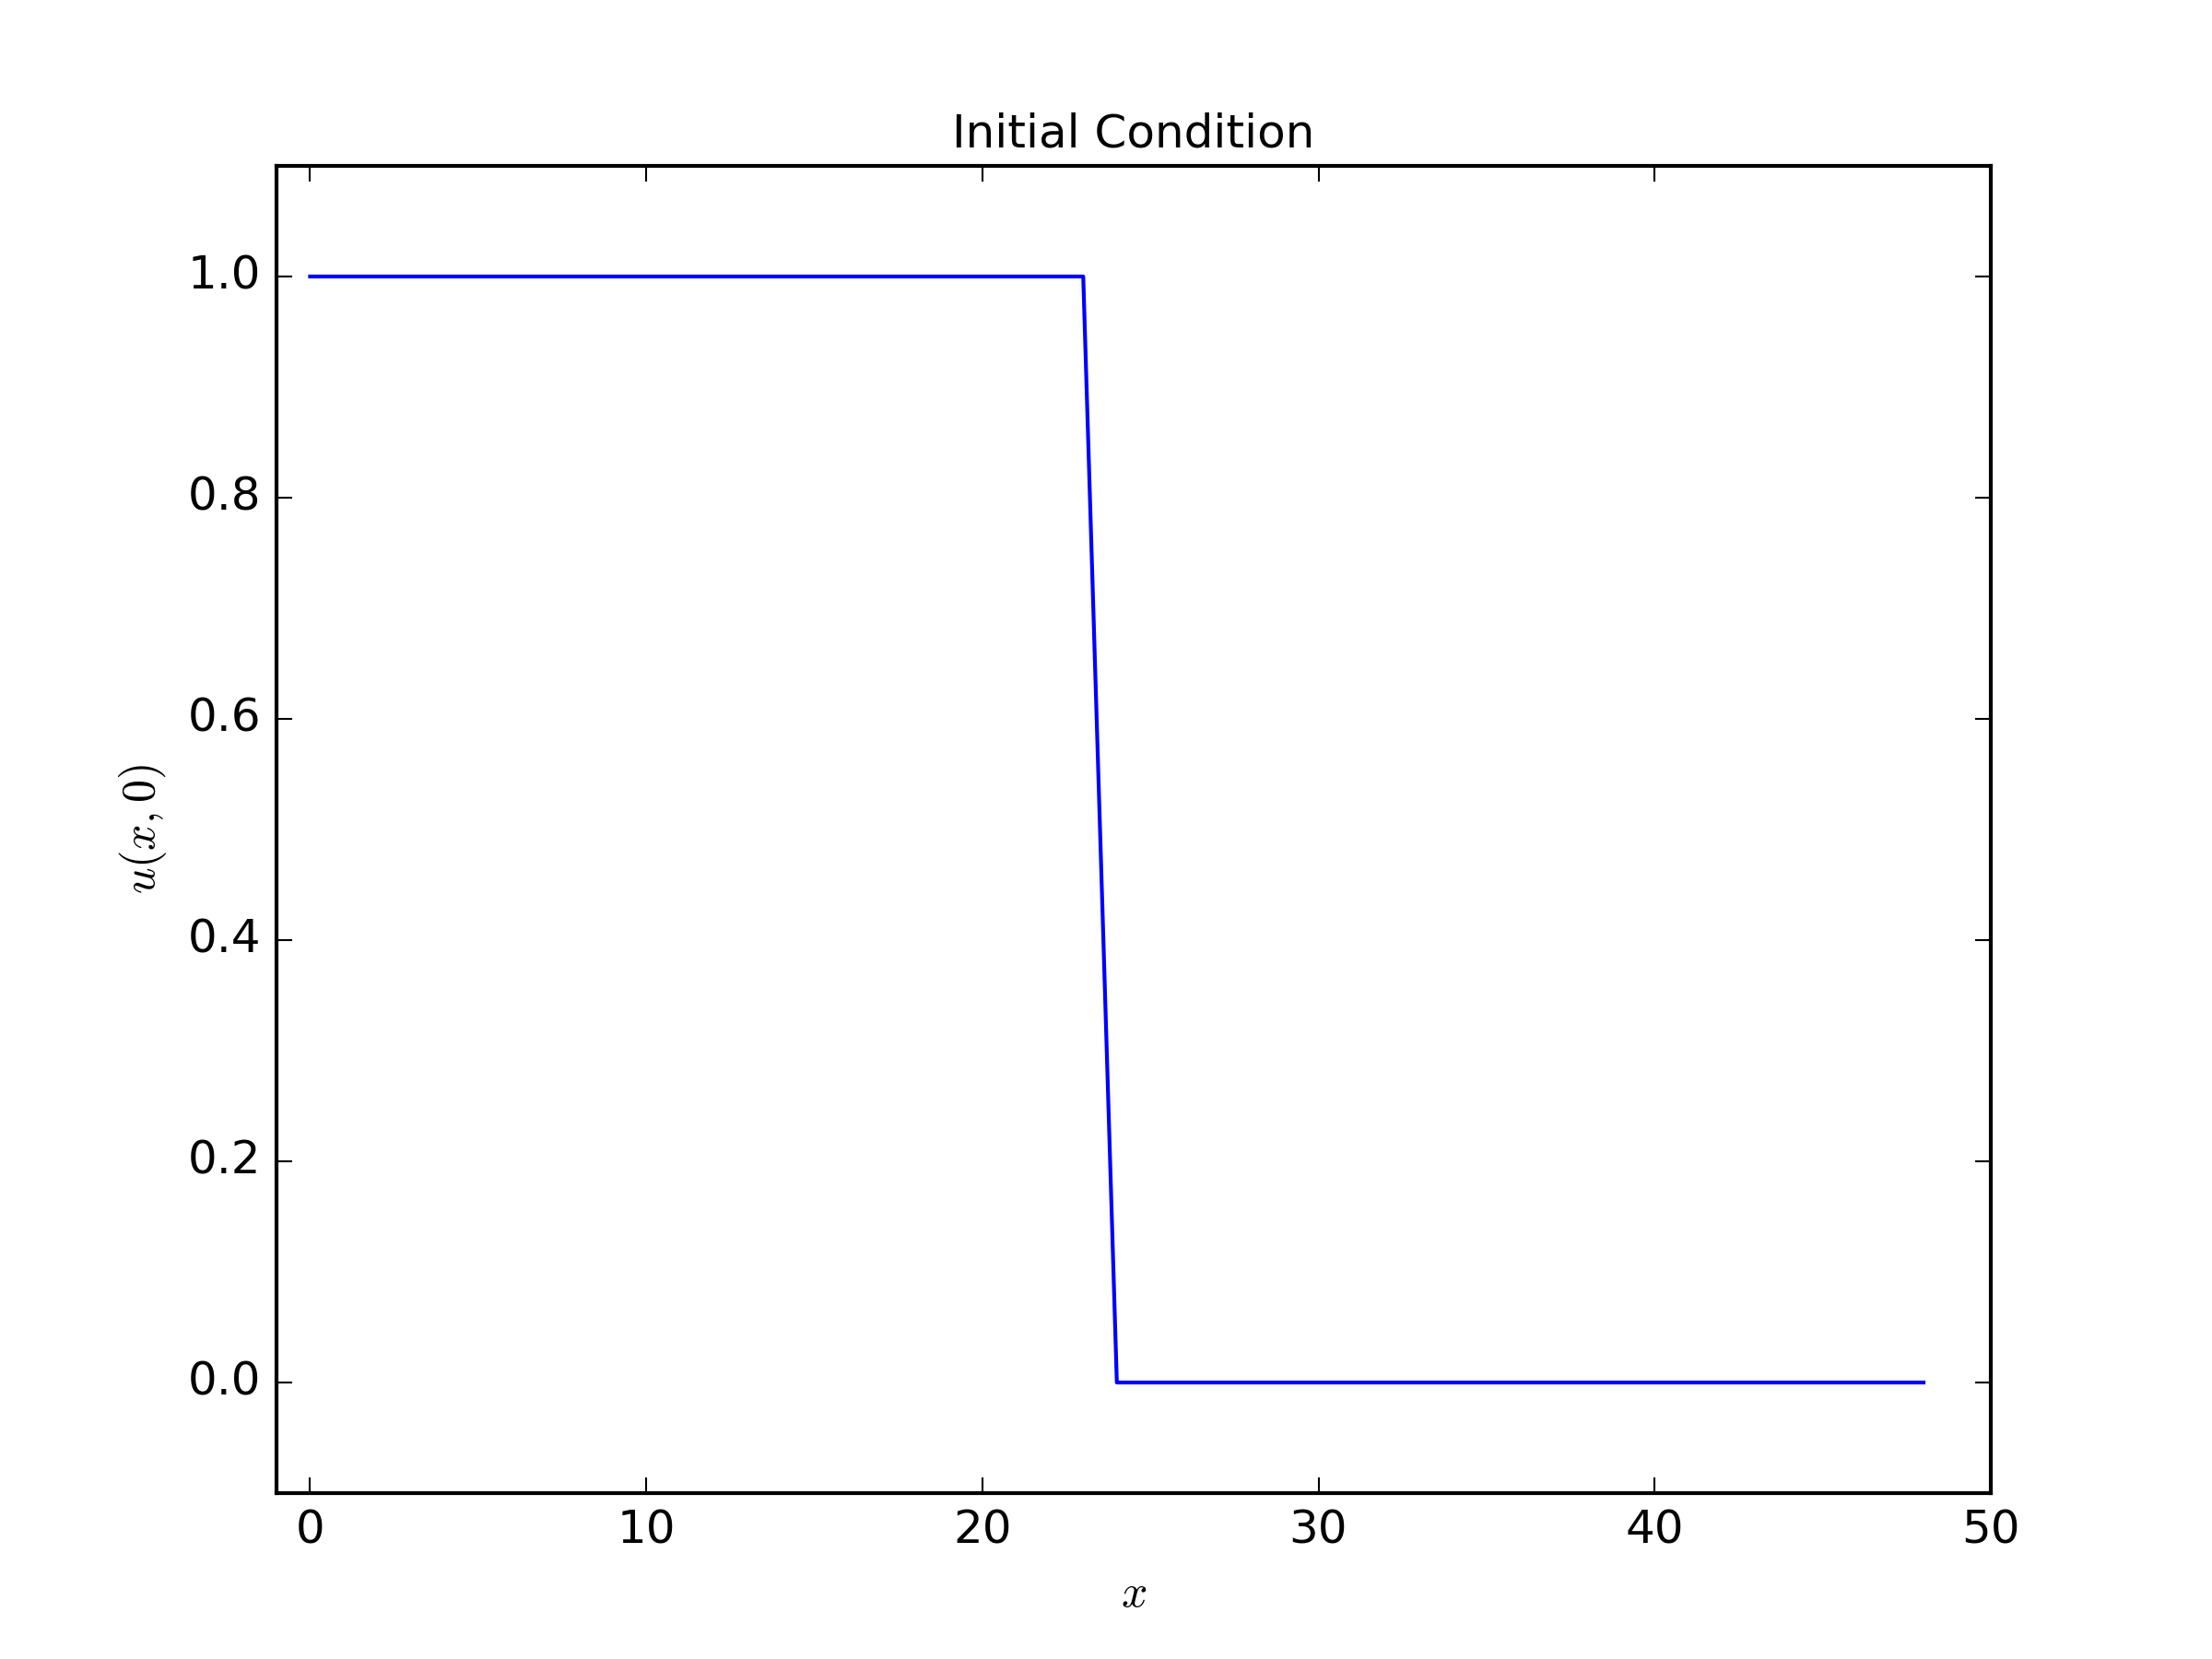
\includegraphics[width=0.75\textwidth]{problem3_initial_condition.png}
\end{figure}

With Crank-Nicolson with grid spacing $\Delta x = 0.02$ and time step $\Delta t = 0.1$, the solution at time $t=1$ develops a noisy disturbance about the discontinuity at $x=0.5$ from the initial condition.

\begin{figure}[H]
\centering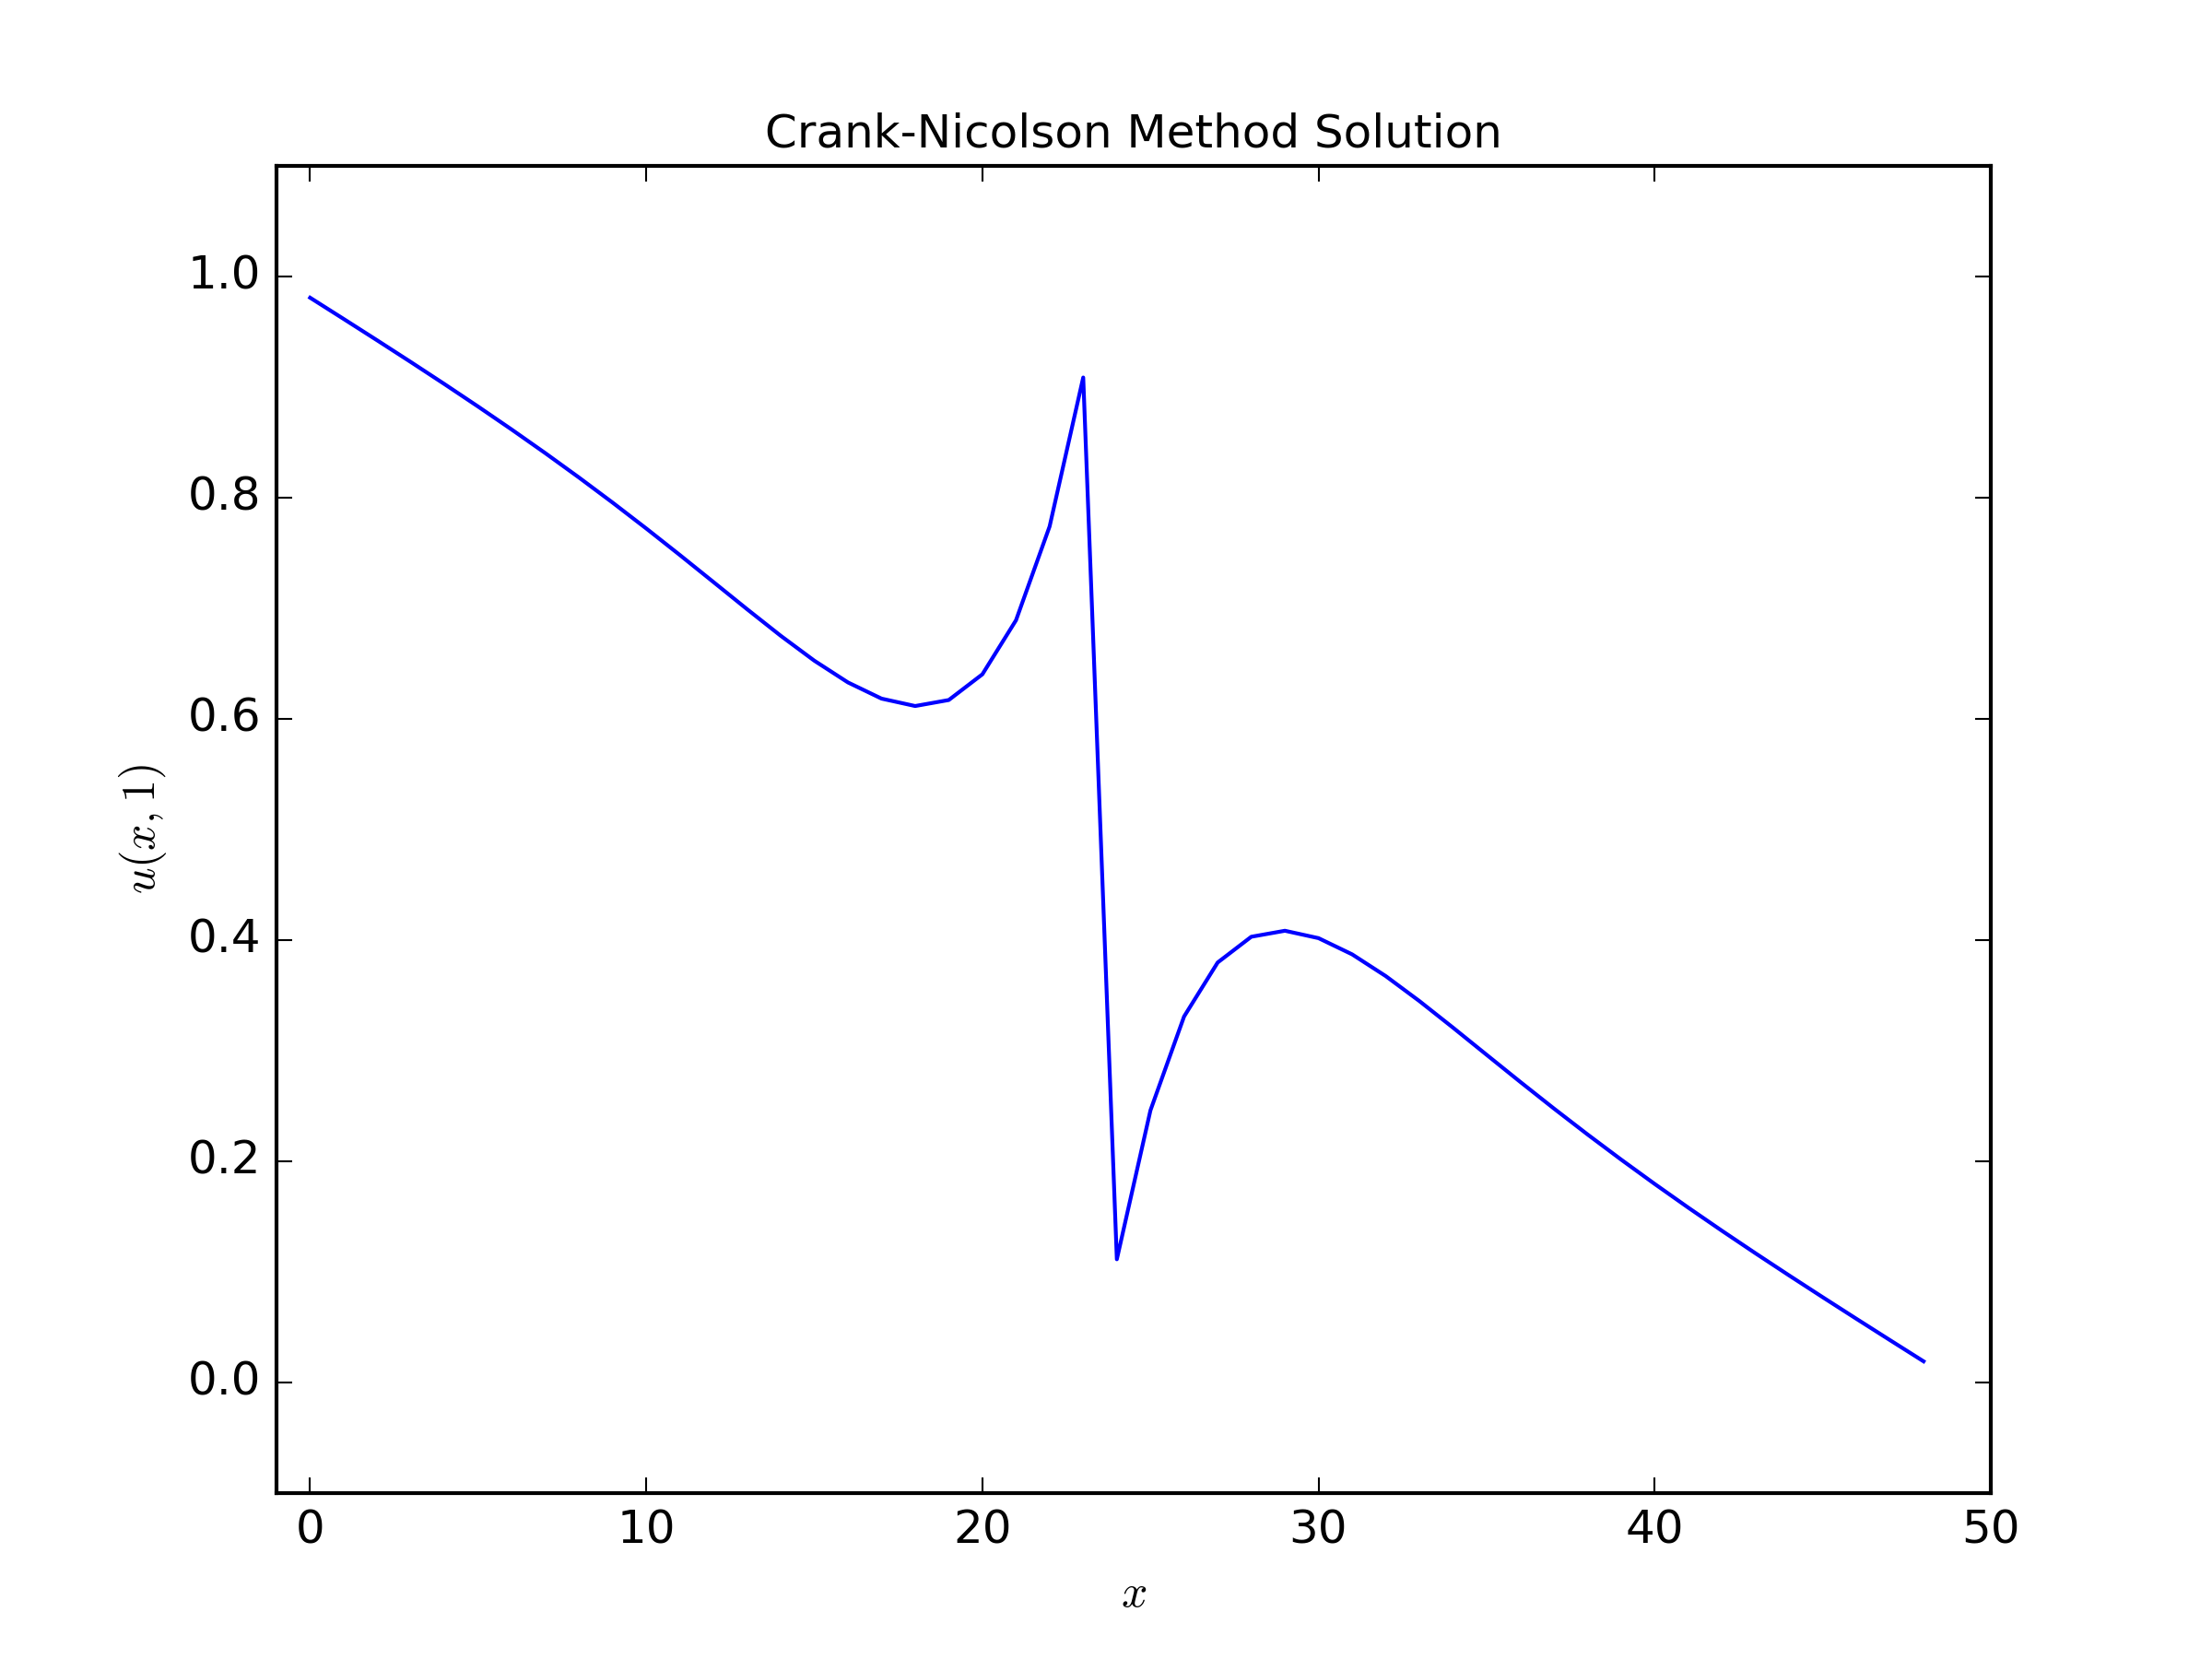
\includegraphics[width=0.75\textwidth]{problem3_crank_nicolson_issue.png}
\end{figure}

\item Give a mathematical argument to explain the unphysical behavior you observed in the numerical solution.

\item Repeat the simulation using BDF2, and discuss why the unphysical behavior is not present in the numerical solution for any time step.
\end{enumerate}

With BDF-2 and the same grid spacing $\Delta x = 0.02$, time step $\Delta t = 0.1$, the solution at time $t=1$ looks smooth and linear as it should.

\begin{figure}[H]
\centering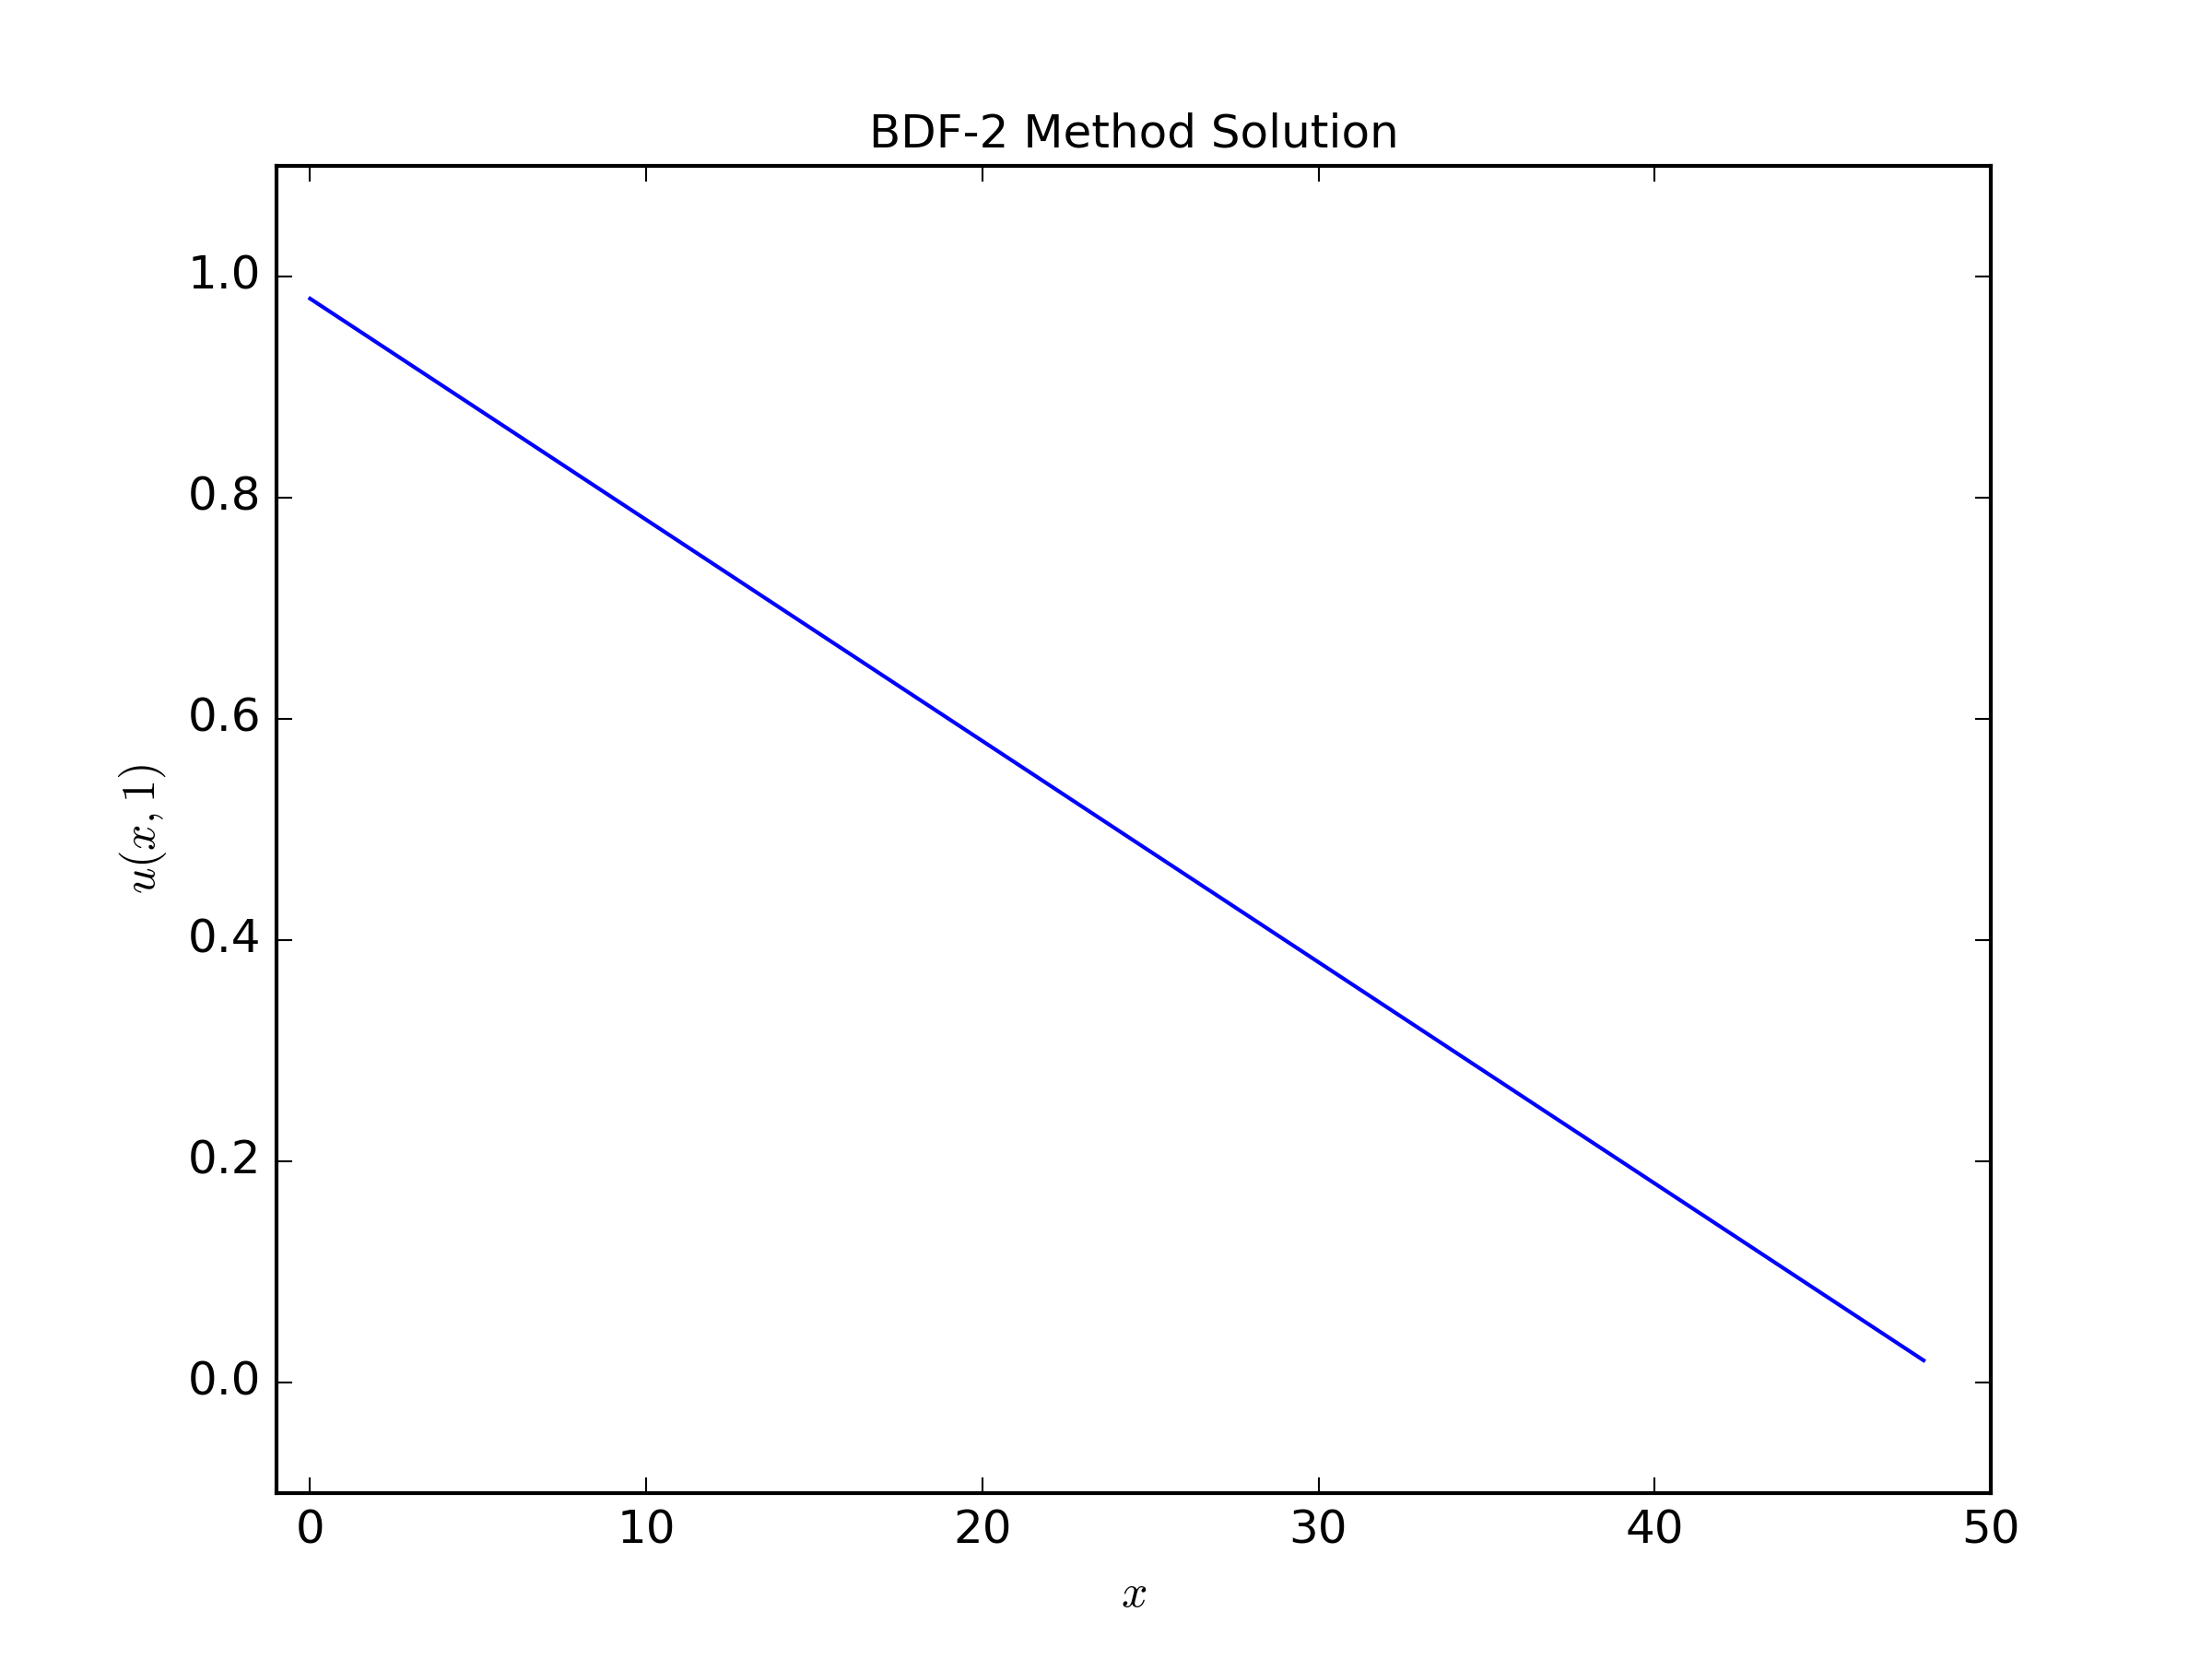
\includegraphics[width=0.75\textwidth]{problem3_bdf2_fixedissue.png}
\end{figure}


\end{document}